\subsection{Definição formal do \textit{market making}}

Os mercados normalmente definem uma quantidade mínima por lote ofertado. Se uma bolsa determina um mínimo de 100 ações um vendedor não poderia criar uma oferta de 50 ações. Se os preços ofertados no momento permitirem a execução de um negócio, a transação ocorrerá em cima da menor quantidade entre as duas ofertas, ou seja, se uma ordem de venda de 100 ações fecha um negócio com uma ordem de compra de 200 ações por exemplo, a quantidade negociada será de apenas 100. O restante da oferta de compra, i.e. 100 ações, continua no livro de oferta de compras, enquanto no lado da venda, a próxima oferta de maior preferência vai para o topo do livro. 

Definimos como $p^{a}$ o preço de uma determinada oferta de venda, chamado de \textit{ask} em inglês e $p^{b}$ para compras, ou \textit{bid} em inglês. Um agente pode ter diversas ofertas para cada ativo $i$, em tempos diferentes indexados pelo símbolo $t$: 
\begin{equation*}
	\begin{aligned}
		p^{a}_{t, i} \text{ para ofertas de venda e}  \\
		p^{b}_{t, i} \text{ para ofertas de compra.}
	\end{aligned}
\end{equation*}

A posição de uma oferta no livro de vendas para um ativo $i$ é dada pela função $\mathbf{pos}_{t, i}^{a}(p) = k$ está na posição $k$ da fila \footnote{onde $k = 0$ é a melhor oferta; com valores de preço decrescentes para vendas, e crescentes para compras.}. A diferença entre ofertas de compra e venda para um mesmo ativo $\Delta_{t, i} = p_{t, i}^{a} - p_{t, i}^{b}$ é o \textit{spread} no momento $t$ e caso $\mathbf{pos}_{t, i}^{a}(p) = \mathbf{pos}_{t, i}^{b}(p) = 0$ é chamado de \textit{bid-ask spread} $\mathbf{\Delta}_{t, i}$.

O objetivo de uma estratégia de \textit{market making} (\textit{MM}) nesse contexto é criar ofertas de compra com valor maior que a melhor oferta, ou menor para ofertas de venda que venham a se tornar as melhores ofertas:

\begin{itemize}
    \item de venda, tais que $p^{a} < P^{a}$; ou 
    \item de compra, tais que $p^{b} > P^{b,}$;
\end{itemize}

onde $p$ é o preço da oferta do agente e $P$ é a melhor oferta existente $\mathbf{pos}_{t, i}^{a}(P) = \mathbf{pos}_{t, i}^{b}(P) = 0$.
É importante notar que quaisquer ordens criadas por um agente de \textit{MM} não geram novas transações no instante \textit{t} (indicado por $p^{a} > P^{b}$ e $p^{b} < P^{a}$ para um mesmo ativo). A seguir um exemplo da reta de preços para um momento $t$ e um ativo $i$ qualquer, onde $p^{b, k}$ é tal que $\mathbf{pos}^{b}(p^{b, k}) = k$:

\begin{figure}
	\begin{center}
		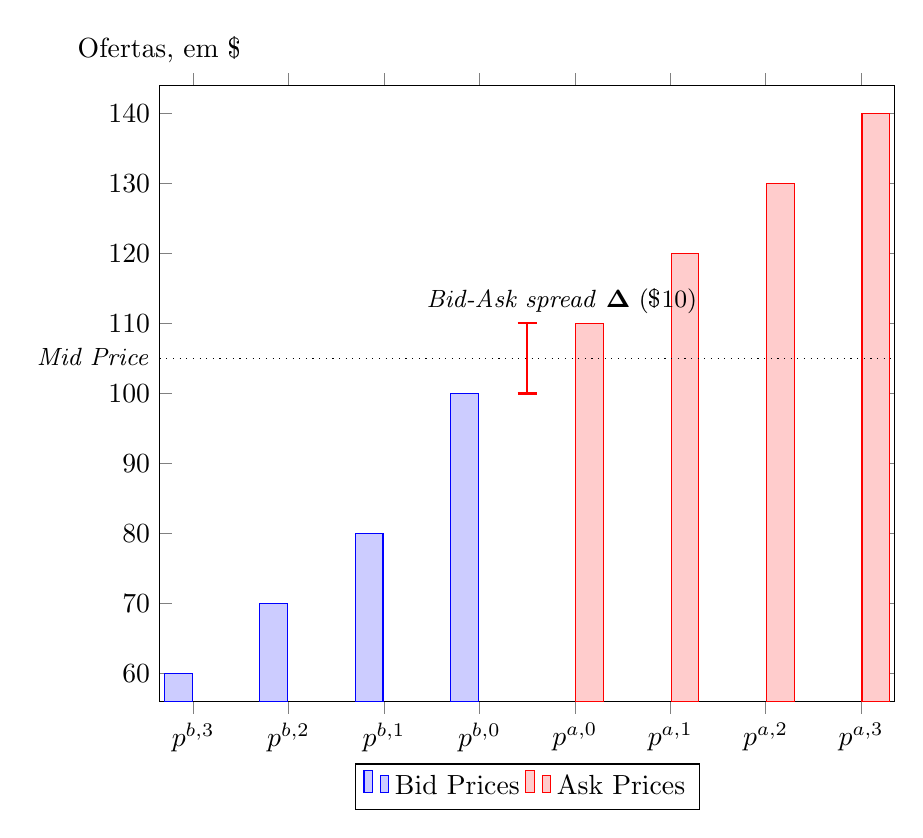
\begin{tikzpicture}
			\begin{axis}[
				x tick label style={/pgf/number format/1000 sep=},
				enlargelimits=0.05,
				legend style={at={(0.5,-0.1)}, anchor=north,legend columns=-1},
				ybar=0.7,
				ylabel={Ofertas, em \$},
    				ylabel style={
    				at={(0,1.02)},
    				anchor=south,
    				rotate=-90,
    			},
				width=0.9\textwidth, % Adjust the width to fit within the box
				xticklabels={
					$p^{b, 3}$, $p^{b, 2}$, $p^{b, 1}$, $p^{b, 0}$, 
					$p^{a, 0}$, $p^{a, 1}$, $p^{a, 2}$, $p^{a, 3}$
					},
				xtick={1,2,3,4,5,6,7,8}, % Set explicit tick positions
				after end axis/.code={
					\draw [red, thick, line cap=] (axis cs:4.5,100) -- (axis cs:4.5,110); % Static vertical line for spread with end caps
					\draw [red, thick] (axis cs:4.4,100) -- (axis cs:4.6,100);
					\draw [red, thick] (axis cs:4.4,110) -- (axis cs:4.6,110);
					\draw [black, dotted] (axis cs:0.65,105) -- (axis cs:8.35,105);
					\node[right, font=\small] at (rel axis cs:0.35,0.65) {\textit{Bid-Ask spread} $\mathbf{\Delta}$ (\$10)}; % Label for the spread line
					\node[left, font=\small] at (rel axis cs:0,0.56) {\textit{Mid Price}};
				}
				]
				% Represent bid prices in blue
				\addplot [blue, fill=blue!20] coordinates {(1, 60) (2, 70) (3, 80) (4, 100)};
				% Represent ask prices in red
				\addplot [red, fill=red!20] coordinates {(5, 110) (6, 120) (7, 130) (8, 140)};
				\legend{Bid Prices, Ask Prices}
			\end{axis}
		\end{tikzpicture}
	\end{center}
	\caption{Gráfico de ofertas de um livro de ordens limite}
\end{figure}

\begin{figure}
	\begin{center}
		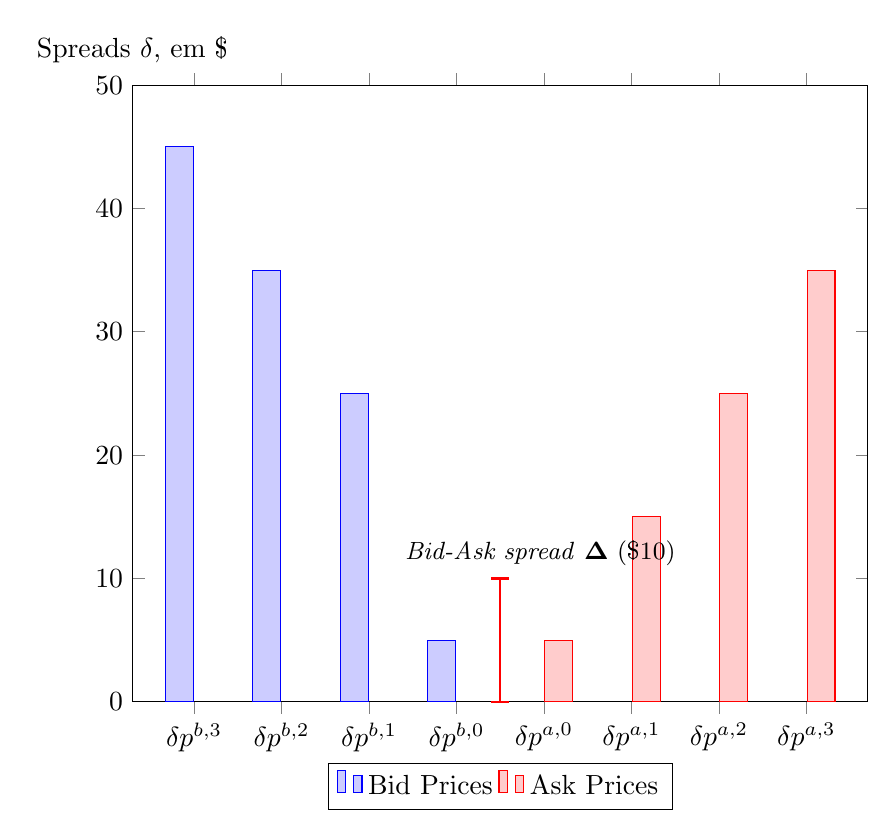
\begin{tikzpicture}
			\begin{axis}[
				x tick label style={/pgf/number format/1000 sep=},
				legend style={at={(0.5,-0.1)}, anchor=north,legend columns=-1},
				ybar=0.7,
				ylabel={Spreads $\delta$, em \$},
				ylabel style={
					at={(0,1.02)},
					anchor=south,
					rotate=-90,
				},
				ymin=0, ymax=50,
				width=0.9\textwidth, % Adjust the width to fit within the box
				xticklabels={
					$\delta p^{b, 3}$, $\delta p^{b, 2}$, $\delta p^{b, 1}$, $\delta p^{b, 0}$, 
					$\delta p^{a, 0}$, $\delta p^{a, 1}$, $\delta p^{a, 2}$, $\delta p^{a, 3}$
					},
				xtick={1,2,3,4,5,6,7,8}, % Set explicit tick positions
				after end axis/.code={
					\draw [red, thick, line cap=] (axis cs:4.5,0) -- (axis cs:4.5,10); 
					% Static vertical line for spread with end caps
					\draw [red, thick] (axis cs:4.4,0) -- (axis cs:4.6,0);
					\draw [red, thick] (axis cs:4.4,10) -- (axis cs:4.6,10);
					\node[right, font=\small] at (axis cs:3.3,12) {\textit{Bid-Ask spread} $\mathbf{\Delta}$ (\$10)}; % Label for the spread line
				}
				]
				% Represent bid prices in blue
				\addplot [blue, fill=blue!20] coordinates {(1, 45) (2, 35) (3, 25) (4, 5)};
				% Represent ask prices in red
				\addplot [red, fill=red!20] coordinates {(5, 5) (6, 15) (7, 25) (8, 35)};
				\legend{Bid Prices, Ask Prices}
			\end{axis}
		\end{tikzpicture}
	\end{center}
	\caption{Gráfico de spreads de um livro de ordens limite}
\end{figure}

Para ilustrar melhor o funcionamento do livro de ordens considere a seguinte situação para um mesmo momento e ativo: um agente qualquer de \textit{MM} tem a \textbf{única oferta de venda} pelo preço de $p^{a}$ no mercado. Caso surja uma nova oferta de \textbf{compra} com melhor preço e acima do preço da oferta do agente $P^{b} \geq p^{a}$, será gerada uma transação pelo preço $p^{a}$ e a ordem de preço $P^{b}$ que gerou a transação é chamada de ordem de mercado, enquanto a ordem do agente é chamada de ordem limite. Após o motor de transações da bolsa receber a ordem com preço $P$, uma transação ocorre e ambas ofertas são removidas do livro de ordens. Em seguida, o agente tem sua posição $r_{t}$ ajustada:
\begin{equation}
    \begin{aligned}
    	r_{t + 1}:= r_{t} + p^{a}q \text{ para vendas e} \\ 
    	r_{t + 1}:= r_{t} - p^{b}q \text{ para compras}
    \end{aligned}
\end{equation}
sendo $r_{t}$ o valor da posição do agente no instante $t$ e $q$ a quantidade de ativos negociadas na transação em questão.

O agente em seguida escolhe esperar ou realizar uma das ações abaixo:
\begin{enumerate}
    \item inserir uma nova oferta de venda, substituindo a oferta anterior;
    \item inserir ou ajustar uma oferta de compra existente no livro de ofertas de compras;
\end{enumerate}

A decisão do agente irá depender de sua expectativa sobre a evolução do mercado, assim como do processo de chegada de ordens de outros agentes, representados pelo identificador $n$, incluindo, mas não limitado à
\begin{itemize}
    \item probabilidade de chegar uma oferta de compra com preço superior $Pr(P_{t + s, i}^{b} > p_{t, i}^{b})$, em algum momento no futuro $s > 0$;
    \item probabilidade de chegar uma oferta de venda com preço inferior $Pr(P_{t + s, i}^{a} < p_{t, i}^{a})$, em algum momento no futuro $s > 0$;
    \item liquidez esperada para o mercado a partir de $t$ até o momento de fechamento do pregão $T$;
    \item risco futuro da posição ultrapassar os limites estabelecidos pelas corretoras.
\end{itemize}

De modo a simplificar as equações adiantes e utilizar uma notação mais comumente usada no contexto de ordens limite, definimos:

\begin{description}[]
	\item[$\delta_{t}(p)$:] $\mathbb{R} \rightarrow \mathbb{R} = |p - p_{t}|$ como a diferença entre o preço $p$ de uma oferta de venda ou compra e o preço de mercado $p$ da ação subjacente no momento $t$.
	
	\item[$\delta_{t}(p, q)$:] $\mathbb{R}^{2} \rightarrow \mathbb{R} = q \cdot \delta_{t}(p)$ como a função que mapeia o impacto de $q$ ações negociadas na carteira do agente sob o \textit{spread} parcial $\delta_t$.
	
	\item[$r_{t}$] é o retorno obtido pelo agente no momento $t$. É calculado pela soma do impacto de todos ativos, onde $s_{t} = \{(p_{t, 0}^{a}, Q_{t, 0}^{a}), ..., (p_{t, n}^{a}, Q_{t, n}^{a}), (p_{t, 0}^{b}, Q_{t, 0}^{b}), ..., (p_{t, m}^{b}, Q_{t, m}^{b})\}$ é o conjunto de ofertas do agente para todos ativos no momento $t$. Cada oferta é uma tupla $(p, Q)$ de preço por ativo e quantidade de ativos ofertada.
	
	\begin{equation} \label{return}
		\begin{aligned}
			r_{t} = \sum_{i = 0}^{n} \delta_{t}(p_{t, i}^{a}, q_{t, i}^{a}) \\
			-\sum_{i = 0}^{m} \delta_{t}(p_{t, i}^{b}, q_{t, i}^{b}) \\
			\forall t < T
		\end{aligned}
	\end{equation}
\end{description}

Onde os valores de  $q$ são as quantidades efetivamente executadas da ordem, podendo ser menor (no caso de uma ordem parcial) ou igual à $Q$ (ordem total), onde $Q$ é a quantidade inicialmente ofertada pelo agente.
Para considerar custos de transação — que incluem tipicamente custos da corretora e emolumentos das bolsas — basta alterar a expressão para $r_{t} := r_{t} - c$, sendo $c$ o custo total de todas transações realizadas.

O agente de \textit{MM}, por fim, observa a sua posição acumulada durante todo o período de negociação $T$ para decidir se obteve retorno positivo ou negativo:
\begin{equation} \label{return_accumulated}
    R_{T} = \sum_{t=0}^{T} r_t
\end{equation}
Define-se matematicamente o valor da posição $R_T$ como a agregação das receitas de vendas, e dos custos de compra e de transações até o momento $T$. 

\subsection{Modelagem do agente de \textit{market making} e do objetivo}
O objetivo principal do agente de \textit{MM} é decidir dentro do intervalo de preços possíveis para uma ação o valor que proporcione o maior retorno para o menor risco associado, de acordo com a fronteira do mercado eficiente \citep{markowitz1952}. O agente também pode decidir a quantidade de ações ofertadas por determinado preço, mas não tem controle direto sobre as quantidades efetivamente negociadas. Ou seja, a quantidade executada $q$ é uma variável estocástica, tal que $P(q = Q), \ \forall q <= Q$ é a probabilidade de que uma oferta de $Q$ ações seja executada por completo em uma ordem. 

Podemos consequentemente modelar o agente como um problema de otimização estocástica com restrições (também chamado de programação estocástica), onde o objetivo inicial do agente é separado em duas etapas: 

\begin{enumerate}[]
	\item maximização do \textit{bid-ask spread} $\mathbf{\Delta}_{t,i} = \delta_{t, i}(p^{a}) + \delta_{t, i}(p^{b}) = |p^{a} - p^{b}|$  para um mesmo ativo;
	
	\item maximização da quantidade executada esperada $\mathbb{E} [q_{t, i}^{a}]$ e $\mathbb{E} [q_{t, i}^{b}]$ de ordens de venda e compra realizadas em cima do maior \textit{bid-ask spread} $\mathbf{\Delta}_{t, i}$, garantindo que a negociação ocorra na fronteira eficiente.
\end{enumerate}

As variáveis de decisão são as combinações possíveis de ofertas de venda e compra — $A$ e $B$\footnote{\ Note que o agente não decide a quantidade executada $q$, apenas a quantidade ofertada $Q$}. A função objetivo do problema é o valor esperado do retorno diário, considerando a incerteza da quantidade executada $q_{i, t} \leq Q_{i}$ por ordem. Substituindo o valor de $q$ na equação \ref{return} pelo seu valor esperado:

\begin{equation}
	\begin{aligned}
		\mathbb{E} [r_{t}] = \sum_{(a, Q) \in A} \delta_{t}(a, \mathbb{E}[q_{a, t}]) \\
		-\sum_{(b, Q) \in B} \delta_{t}(b, \mathbb{E}[q_{b, t}]) \\
		\forall t < T
	\end{aligned}
\end{equation}
e o retorno diário acumulado da equação \ref{return_accumulated} é utilizado como função objetiva que se deseja maximizar:
\begin{equation}
	\begin{aligned}
		\max_{A, B} \quad & \sum_{t=0}^{T} \ \mathbb{E} [r_{t}]
	\end{aligned}
\end{equation}

De modo a obter uma solução para a otimização estocástica definimos o agente como um processo de decisão de Markov $(\mathcal{S}, \mathcal{A}, T, r)$, buscando modelar o problema para o paradigma de Aprendizado por Reforço:

\begin{description}
	\item[$\mathcal{S}$] 
	é o espaço de estados possíveis, representado pelo conjunto $\{(A_{t}, B_{t}, L_{t}) \ | \ t < T\}$, onde cada estado $s \in \mathcal{S}$ é uma combinação possível de ofertas de venda e de compra do agente, e o livro de ordens limite no momento $t$;
	\item[$\mathcal{A}$] é o espaço de ações que o agente pode realizar, ou seja, a combinação de novos \textit{spreads} $\delta(a_{i})$ e novas quantidades $Q^{+}_{i}$ (ou $Q^{-}_{i}$ caso a quantidade ofertada diminua) que atualizem os conjuntos $A$ e $B$ de ofertas de venda e compra existentes.
	\item[\textit{T}] são as transições possíveis entre estados dado uma ação tomada pelo agente. São representadas pela função de transição $T :  \mathcal{S} \times \mathcal{A} \times \mathcal{S} \rightarrow [0, 1]$, que mapeia o estado atual e a ação tomada para a probabilidade de ir para um estado subjacente. No caso do agente de \textit{market-making}, a função $T$ recebe o estado atual $s$ e a ação $a$ tomada pelo agente (conjunto de \textit{spreads} e quantidades ofertadas atualizadas). Em seguida recebe um possível estado futuro $s' \in \mathcal{S}$ e retorna a probabilidade de transição $T(s, a, s') = Pr(S_{t+1} = s' \ | \ S_{t} = s, A = a)$.
	\item[\textit{r}] é a função de recompensa da cadeia aleatória, que mapeia o estado atual e a ação do agente para a probabilidade de uma recompensa ocorrer caso a transição para um determinado estado seguinte ocorra.
\end{description}

Utilizando a definição do agente como um Processo de Decisão de Markov (MDP), podemos empregar uma abordagem de Aprendizado por Reforço (RL) para simular o ambiente e encontrar uma política de decisão de preços ótimas. Esta seção explora em detalhes como o Aprendizado por Reforço é aplicado a esse contexto desafiador e por que essa abordagem é crucial.

\begin{itemize}
	\item Trajetória ($\tau$): é a sequência de estados observados e ações tomadas ao longo do tempo. No contexto de \textit{MM}, uma trajetória consiste em uma série de estados do mercado $s_{t} = (A_{t}, B_{t}, L_{t})$ seguidas da ação em cima desse estado $a_{t} = \{(\delta_{t}(p_{i}), Q_{i}) \ | \ \forall i \}$. Essas trajetórias representam a jornada do agente no mercado financeiro, incluindo suas ações e interações com o ambiente.
	
	\[
	\tau = (s_0, a_0, s_1, a_1, \ldots, s_T, a_T)
	\]
	
	Onde \(s_t\) é o estado no tempo \(t\), e \(a_t\) é a ação tomada no tempo \(t\).
	
	\item Política ($\pi$): função que mapeia o estado atual (\textit{spreads} $\delta$ e quantidades $Q$) para a escolha de ações (ofertas de compra e venda). Através de algoritmos de otimização de decisão (\textit{Policy Optimization} e \textit{Q-Learning}), nosso objetivo é encontrar uma política ótima que permita ao agente tomar decisões que maximizem seus retornos no mercado. Essa política é fundamental para determinar como o agente se comporta em diferentes situações de mercado.
	
	\[
	\pi(s) \rightarrow a
	\]
	
	Essa função determina como o agente toma decisões em diferentes estados.
	
	\item Função de Valor ($V$): estima o valor esperado acumulado que o agente pode obter ao seguir a política \(\pi\) a partir de um estado inicial. No contexto do agente de market making, \(V\) depende do preço de venda \(a\) e da quantidade \(Q\), bem como da política do agente. Através do Aprendizado por Reforço, podemos calcular \(V\) para avaliar quão bom é um estado, o que orienta o agente na seleção de ações que maximizam seu desempenho global.
	
	\begin{equation*}
		V(s_0) = \mathbb{E}\left[\sum_{t=0}^{T} \gamma^t \cdot r(s_t, \pi(s_t)) \right]
		\end{equation*}
		
	Onde \(\gamma\) é o fator de desconto que pondera as recompensas futuras, e a expectativa é tomada sobre todas as possíveis trajetórias do agente.
\end{itemize}


**Por que fazer isso?**

A aplicação do Aprendizado por Reforço nesse cenário é de suma importância por diversas razões:

- **Tomada de Decisão Ótima:** Através da aprendizagem de uma política de decisão ótima, o agente pode aprimorar suas estratégias de negociação, maximizando seus lucros em um ambiente financeiro complexo e estocástico.

- **Adaptação a Mudanças:** O Aprendizado por Reforço permite que o agente se adapte a mudanças nas condições de mercado ao longo do tempo, tornando-o mais resiliente a flutuações e incertezas.

- **Eficiência e Aplicação em Tempo Real:** Uma vez treinado, o agente pode ser usado para tomar decisões em tempo real no mercado financeiro, proporcionando uma vantagem competitiva para instituições financeiras e traders.

- **Contribuição à Pesquisa:** A modelagem de um agente de market making como um MDP e a aplicação de RL contribuem para o avanço da pesquisa em finanças quantitativas e aprendizado de máquina, abrindo novas possibilidades para o desenvolvimento de estratégias de negociação mais eficientes e robustas.

Essa abordagem combina os princípios do Aprendizado por Reforço com o complexo cenário do mercado financeiro, permitindo ao agente aprimorar suas habilidades de negociação e, ao mesmo tempo, contribuir para o progresso da pesquisa em finanças quantitativas.

De modo a tornar o agente adverso ao risco noturno, insere-se também uma restrição adicional, de que ao final do dia não haja exposição a riscos de mercado. 
Existem algumas alternativas para formalizar matematicamente essa restrição:
\begin{enumerate}
    \item No final do dia, o agente não pode ter nenhum ativo em posição: 
    \begin{equation}
        \sum_{b=1}^{B_t} q_b  - \sum_{a=1}^{A_t} q_a = 0\label{eq:eod_restriction}
    \end{equation}
    \item No final do dia, se houver alguma posição, o agente precisa \textit{headgear} a exposição ao risco, comprando (vendendo) futuros ou outros derivativos, dependendo da posição remanescente.\footnote{De maneira simplificada, o \textit{hedge} consiste em comprar ou vender ativos que tenham uma exposição ao risco oposta aos riscos da carteira atual, de modo a equilibrar a posição.}
\end{enumerate}

\subsection{\textit{Market making} simultâneo}
Ao considerarmos a situação em que o MM aplica a sua estratégia em diversos mercados simultaneamente observamos um aumento da complexidade, mas também das alternativas para lidar com riscos envolvidos - chamamos essa situação de MM \textbf{simultâneo} ou \textbf{multivariado}.

Para tal, a posição $V_{T}$ do agente passa a ser a soma de todas posições parciais $V_{T, k}$, onde $k$ é uma bolsa onde o agente possui ações:
\begin{eqnarray*}
    V_t &=& \sum_{k=1}^N V_{T, k}\\
\end{eqnarray*}

O objetivo principal (\ref{eq:target_fct}) continua o mesmo, e mantém-se a restrição (\ref{eq:eod_restriction}). Contudo, surgem novas alternativas para proteção da carteira durante a noite:

\begin{enumerate}
    \item O agente pode avaliar o risco global da carteira, e incluir um único ativo de proteção contra o risco global ao final do dia.
    \item Se o ativo for negociado em múltiplas bolsas (chamado também de ativo \textit{co-listed}), o agente pode continuar a negociação deste em outra bolsa caso uma delas esteja fechada.
\end{enumerate}

Considerando um cenário em que haja ações em \textit{co-listing}, surge a possibilidade de criação de estratégias mais sofisticadas, permitindo a implementação dos itens mencionados acima.
 